\begin{figure*}[h!]
\centering
\begin{adjustwidth}{-1em}{-1em}
\vspace*{-1ex}
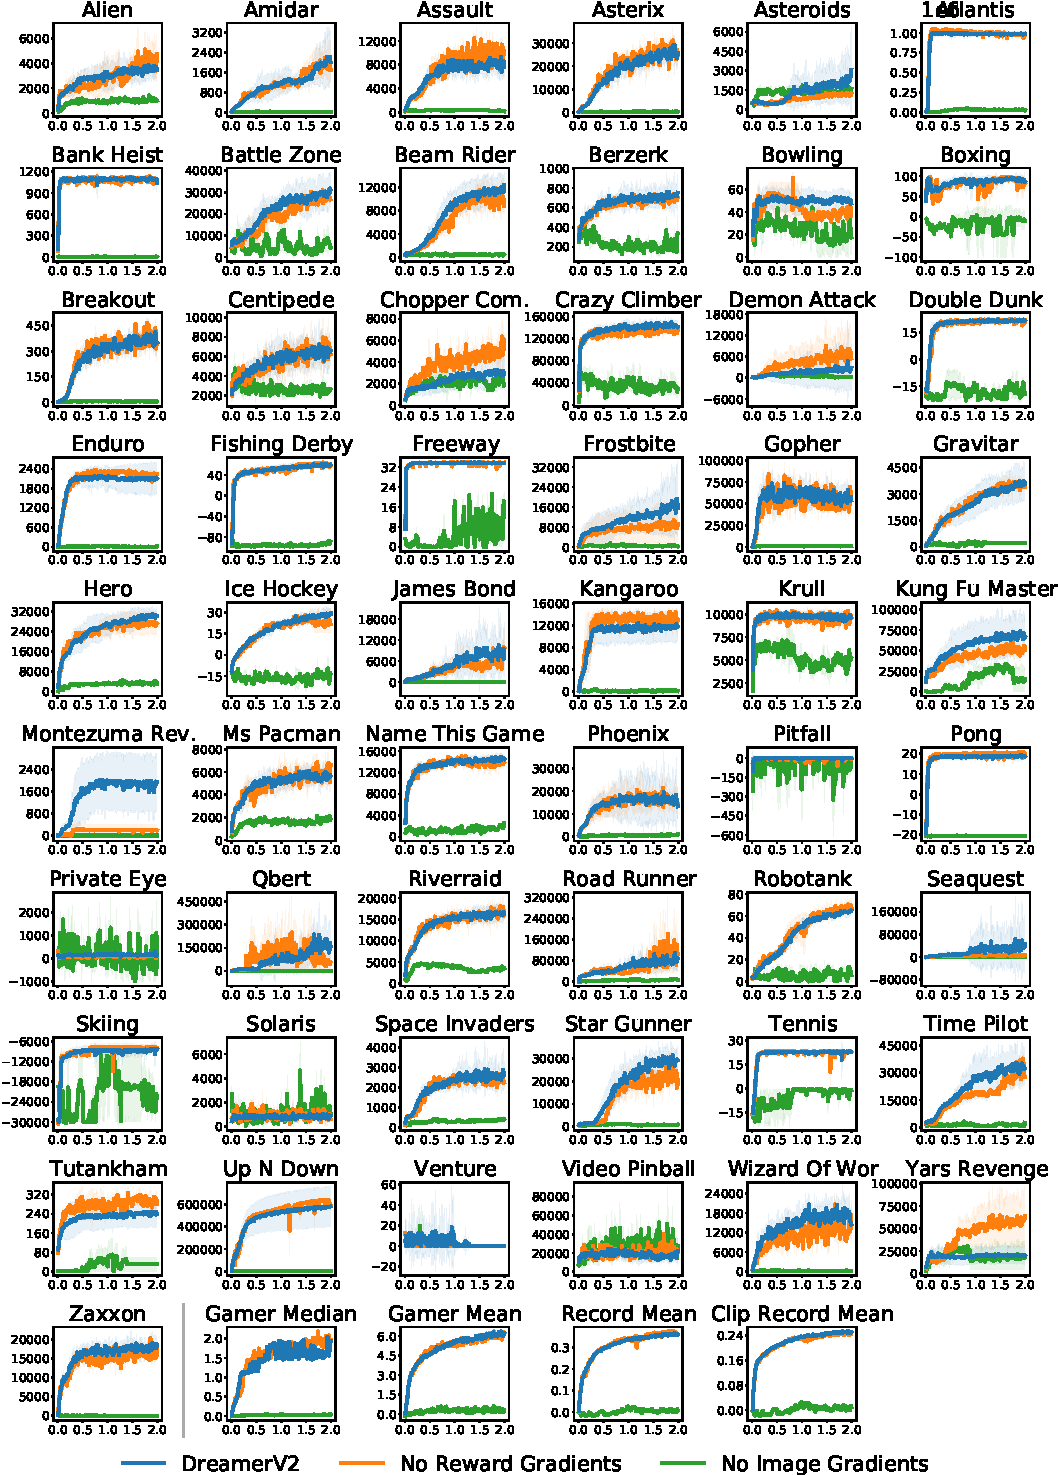
\includegraphics[width=\linewidth]{tasks-repr/tasks-repr}
\end{adjustwidth}
\caption{Comparison of leveraging image prediction, reward prediction, or both for learning the model representations. While image gradients are crucial, reward gradients are not necessary for our world model to succeed and their gradients can be stopped. Representations learned purely from images are not biased toward previously encountered rewards and outperform reward-specific representations on a number of tasks, suggesting that they may generalize better to unseen situations.}
\label{fig:tasks-repr}
\vspace*{-2ex}
\end{figure*}
